\documentclass[10pt, xcolor={dvipsnames}, sans, mathserif, aspectratio=169]{beamer}

\usepackage{fontspec}
\usepackage{fontawesome5}
\usepackage{mathrsfs}
\usepackage{amsmath, amssymb}
\usepackage{braket}
\usepackage{graphicx}
\usepackage{hyperref}
\usepackage[absolute,overlay]{textpos}
\usepackage[font=tiny, skip=0.1pt]{caption}
\usepackage[dvipsnames]{xcolor}
\usepackage{mathtools}
\usepackage[backend=bibtex, style=science]{biblatex}

\graphicspath{{./imgs/}}

\captionsetup[figure]{labelformat=empty}

% Define the custom theme
\mode<presentation>
{
\usefonttheme{serif}
% \setmainfont{DejaVu Sans Mono}
% \setbeamertemplate{page number in head/foot}[totalframenumber]
\setbeamertemplate{footline}[frame number]
\setbeamertemplate{caption}[default]
\setbeamertemplate{navigation symbols}{}

\setbeamerfont{footnote}{size=\tiny}
}

% Some custom commands
\newenvironment{List}[2]
{\begin{textblock}{#1}#2
\begin{itemize}}
{\end{itemize}
\end{textblock}}

\newenvironment{Pic}[2]
{\begin{textblock}{#1}#2
\begin{figure}}
{\end{figure}
\end{textblock}}

\addbibresource{aps-dnp-2024-refs.bib}

\newcommand{\citeslide}[1]{{\tiny \footfullcite{#1}}}

% Title of the slides
\title{Deep-Learning Unfolding for Extraction of Drell-Yan Angular Parameters in $pp$ Collisions with 120 GeV Beam Energy}
% \subtitle{Subtitle}
\author{Dinupa Nawarathne}
\institute{New Mexico State University \\
Representing the FermiLab SeaQuest/E906 Collaboration
}

\date{APS-DNP-2024, October 10, 2024}

\titlegraphic{

\includegraphics[height=0.8cm]{imgs/Fermilab_logo.svg.png}

\includegraphics[height=0.8cm]{imgs/NMSU_logo.jpg}

\includegraphics[height=0.8cm]{imgs/SeaQuest.jpg}

\includegraphics[height=0.8cm]{imgs/DOE.png}
}

\begin{document}

\begin{frame}
    \maketitle
\end{frame}

\begin{frame}
\frametitle{Drell-Yan Process}

\begin{Pic}{6.}{(0.5, 2.)}
	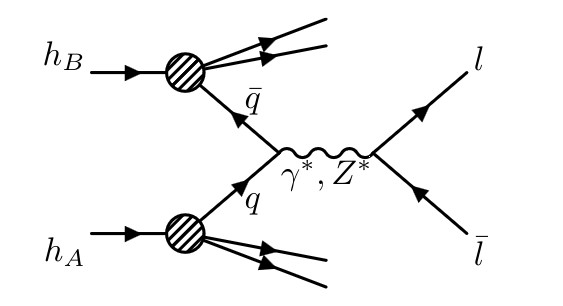
\includegraphics[width=5.9cm]{drell-yan.png}
	\caption{Drell-Yan process\citeslide{Bechtel:2009zza}}
\end{Pic}

\begin{textblock}{8.}(7., 0.5)
\begin{equation*}
\dfrac{d\sigma}{d\Omega} = 1 + \lambda \cos^{2}\theta + \mu \sin2\theta\cos\phi + \dfrac{1}{2}\nu\sin^{2}\theta\cos2\phi
\end{equation*}
\end{textblock}

\begin{Pic}{4.}{(7., 2.1)}
	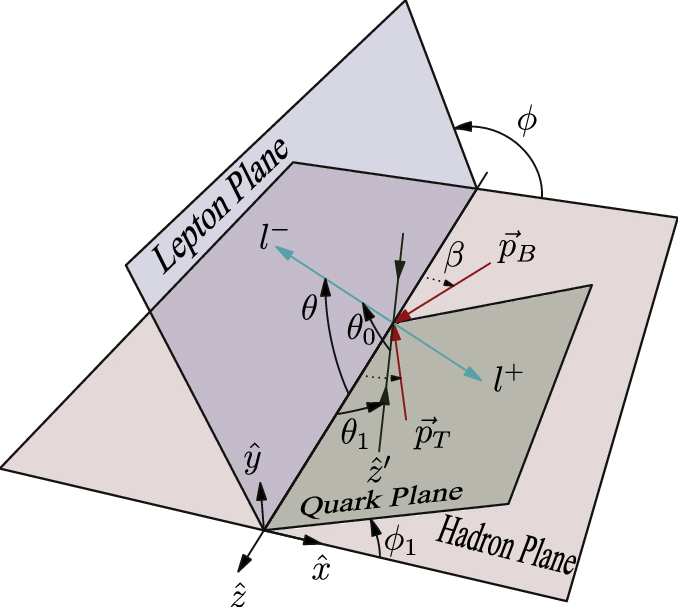
\includegraphics[width=3.9cm]{collins-soper-frame.png}
	\caption{Collins-Soper frame: rest frame of the dileptons\citeslide{Peng:2018tty}}
\end{Pic}

\begin{List}{10.}{(0.5, 9.7)}
	\item $\lambda$, $\mu$ and $\nu$ - angular coefficients of the lepton angular distribution.
	
	\item Non-zero $\nu$ parameter provide information about the transverse motion of the quarks inside the proton.
\end{List}

\begin{Pic}{5.}{(11., 6)}
	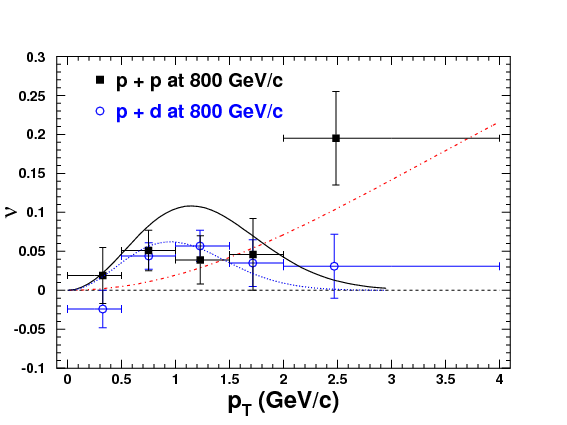
\includegraphics[width=4.9cm]{nu-e866.png}
	\caption{Extraction of $\nu$ parameter in FermiLab-E866/NuSea experiment\citeslide{NuSea:2008ndg}. Curves are theoretical calculations.\citeslide{PhysRevD.77.054011}}
\end{Pic}

\end{frame}

\begin{frame}
\frametitle{FermiLab SeaQuest/E906 Experiment}

\begin{Pic}{8.}{(0.5, 2.)}
	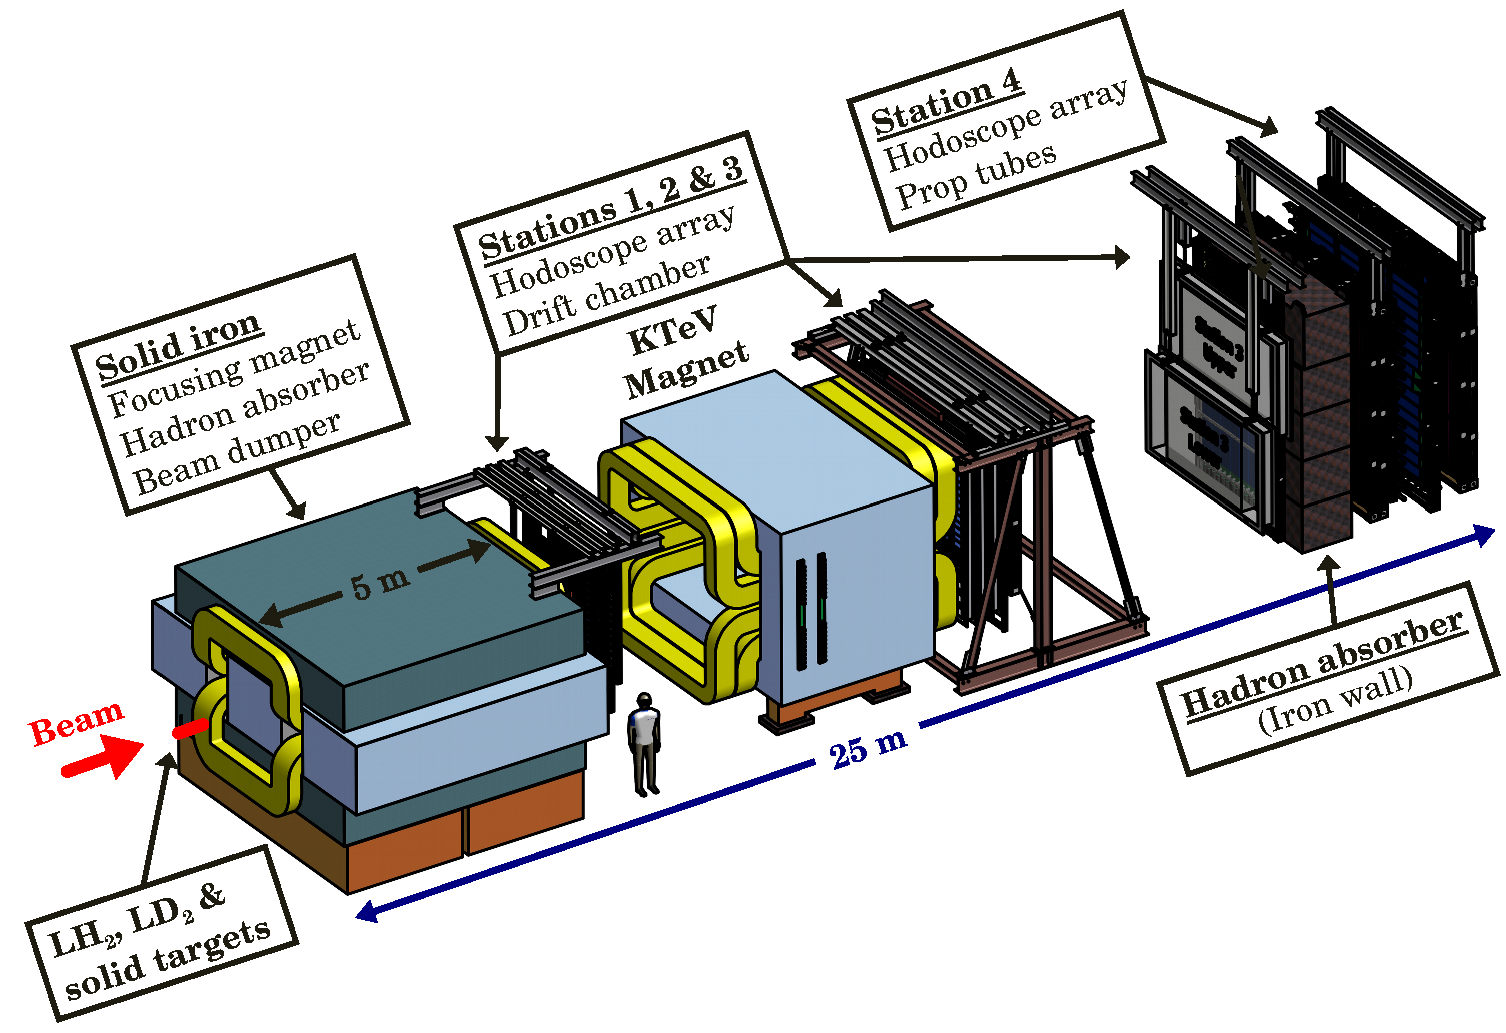
\includegraphics[width=7.9cm]{spectrometer.pdf}
	\caption{SeaQuest spectrometer\citeslide{SeaQuest:2017kjt}}
\end{Pic}

\begin{List}{6.}{(0.5, 2.)}
	\item Fixed target experiment at FermiLab
\end{List}

\begin{Pic}{7.}{(9., 1.)}
	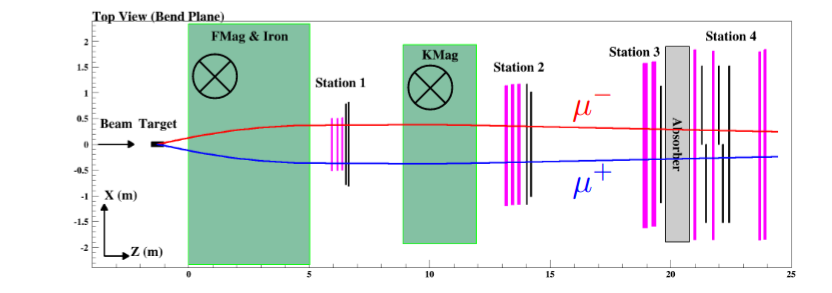
\includegraphics[width=6.9cm]{mup-mum.png}
	\caption{$\mu^{+/-}$ tracks\citeslide{Nagai:2017fcp}}
\end{Pic}

\begin{List}{7.}{(9., 7.)}
	\item Use 120 GeV beam energy from main injector.
	
	\item Main goal is to measure the antiquark structure of the nucleon.
	
	\item SeaQuest data is capable of extracting the Drell-Yan angular coefficients.
\end{List}

\end{frame}

\begin{frame}
\frametitle{Analysis Pipeline}

\begin{Pic}{0.}{(1., 2.)}
	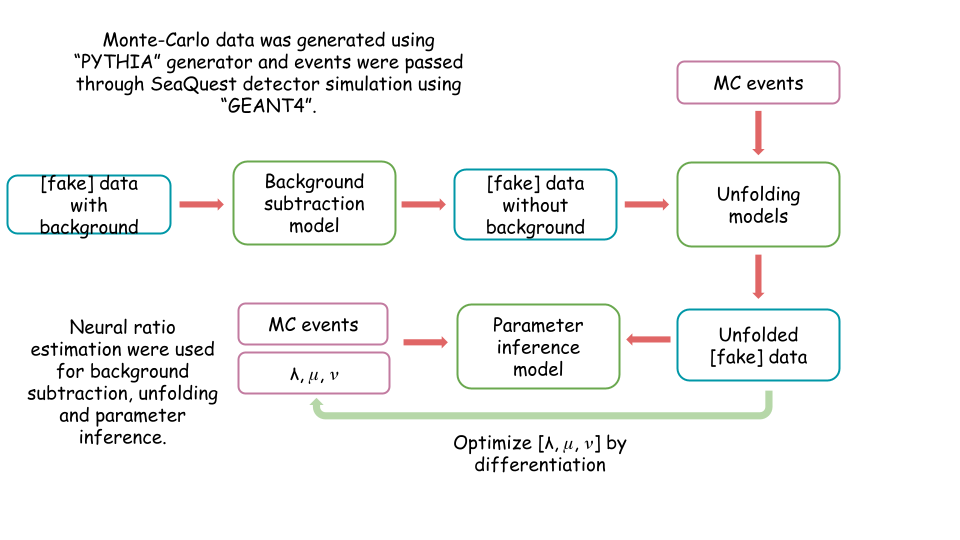
\includegraphics[width=15.cm]{pipeline.png}
\end{Pic}
\end{frame}

\begin{frame}
\frametitle{Neural Likelihood Ratio Estimation}

\begin{List}{15.}{(0.5, 2.)}
	
	\item Consider two joint probability distributions of the Drell-Yan process $p(\phi, \cos\theta | \lambda_{1}, \mu_{1}, \nu_{1})$ and $p(\phi, \cos\theta | \lambda_{0}, \mu_{0}, \nu_{0})$. Then the likelihood ratio is given by,
	
	\begin{equation*}
		\mathcal{L} = \dfrac{p(\phi, \cos\theta | \lambda_{0}, \mu_{0}, \nu_{0})}{p(\phi, \cos\theta | \lambda_{1}, \mu_{1}, \nu_{1})}
	\end{equation*}
	
	\item Let $f(\phi, \cos\theta)$ be a classifier trained to classify between two equal-sized samples ${\phi, \cos\theta} \sim p(\phi, \cos\theta | \lambda_{0}, \mu_{0}, \nu_{0})$, labeled $y = 0$ and ${\phi, \cos\theta} \sim p(\phi, \cos\theta | \lambda_{1}, \mu_{1}, \nu_{1})$, labeled $y = 1$. Then likelihood ratio estimator can be defined as;
	
	\begin{equation}
		\hat{r}(\phi, \cos\theta) = \dfrac{1 - f(\phi, \cos\theta)}{f(\phi, \cos\theta)}
		\label{eq:1}
	\end{equation}
	
	\item We can use equation \ref{eq:1} as a reweighting method;
	
	\begin{equation*}
		p(\phi, \cos\theta | \lambda_{0}, \mu_{0}, \nu_{0}) \approx \hat{r}(\phi, \cos\theta) p(\phi, \cos\theta | \lambda_{1}, \mu_{1}, \nu_{1})
	\end{equation*}
	
	i.e. even if the analytical formula for the likelihood ratio is intractable, we can approximate the likelihood ratio between two joint probability distributions.\citeslide{Brehmer:2018eca}
	
\end{List}
\end{frame}

\begin{frame}

\begin{Pic}{6.}{(0., 0.5)}
	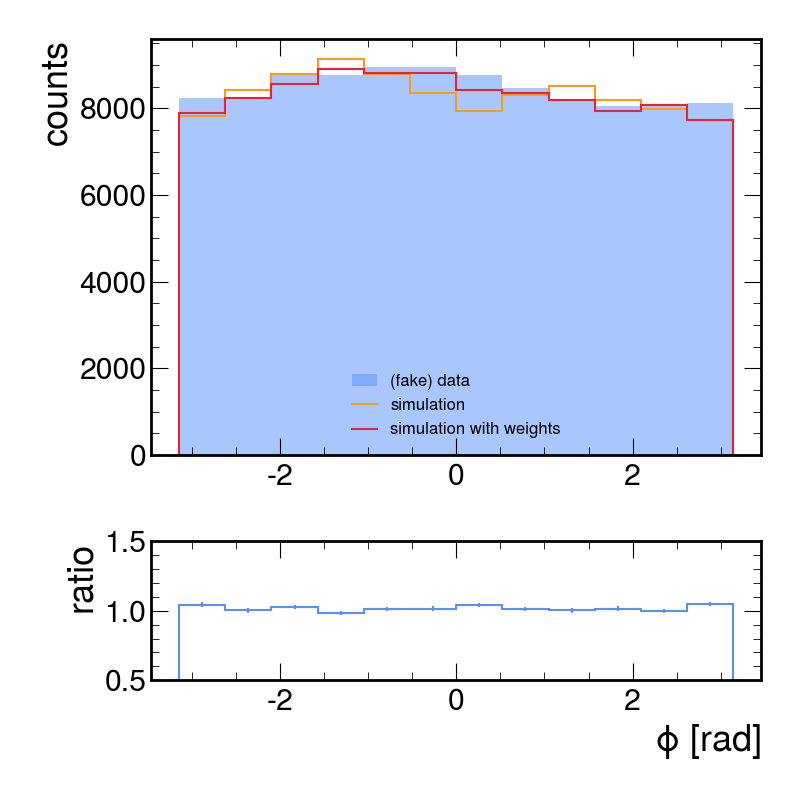
\includegraphics[width=5.9cm]{phi.png}
\end{Pic}

\begin{Pic}{5.}{(6., 0.5)}
	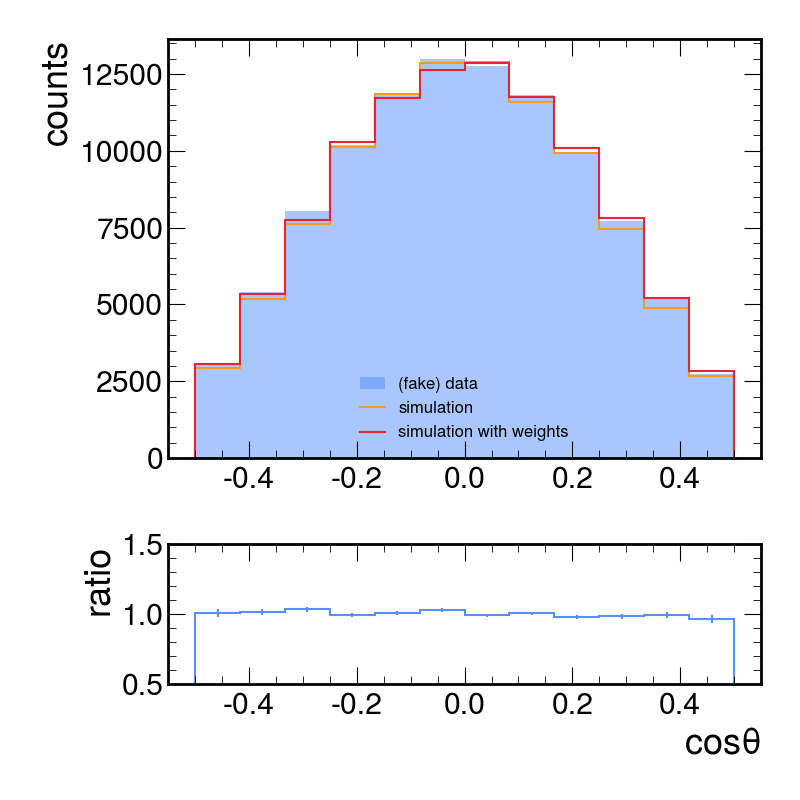
\includegraphics[width=4.9cm]{costh.png}
\end{Pic}

\begin{Pic}{5.}{(11., 0.5)}
	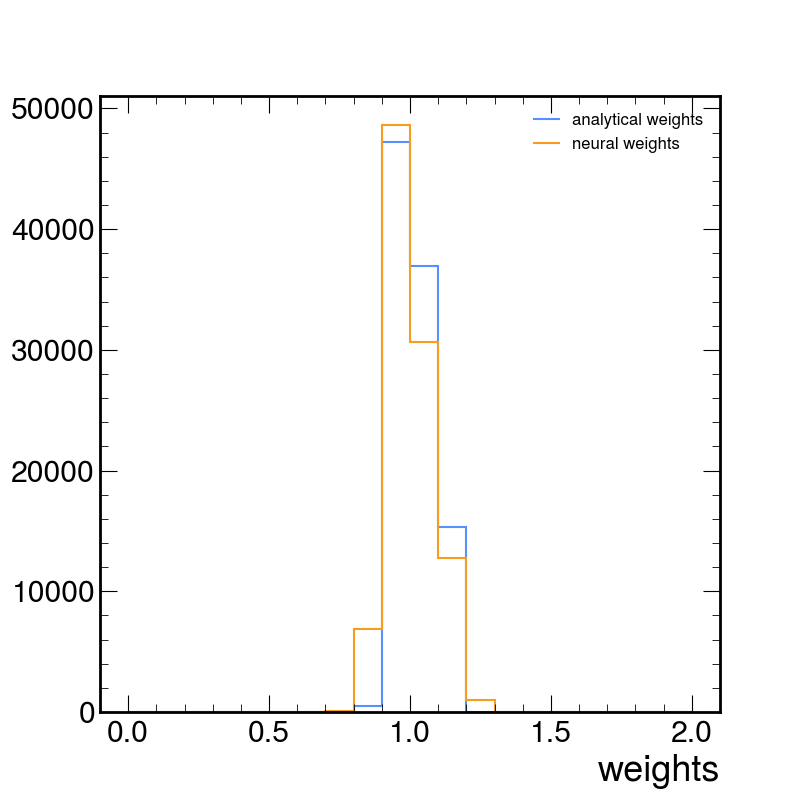
\includegraphics[width=4.9cm]{weights.png}
\end{Pic}

\begin{textblock}{15.}(0.5, 11.)
	In this example we choose values $[\lambda_{1}, \mu_{1}, \nu_{1}] = [1., 0., 0]$ and $[\lambda_{0}, \mu_{0}, \nu_{0}] = [0.9, -0.2, 0.1]$. Reconstructed $\phi$ and $\cos\theta$ are used as inputs to the neural network. The weights calculated using the neural ratio estimator show good agreement with the analytically derived weights. We will employ this method for reweighting in background subtraction, unfolding, and parameter inference.\citeslide{Brehmer:2019xox}
\end{textblock}

\end{frame}

\begin{frame}
\frametitle{Background Subtraction}

\begin{List}{15.}{(0.5, 1.5)}
	
	\item Fist we need to subtract the background\footnote{In SeaQuest experiment is dominated by combinatoric background and estimated by event mixing method}\citeslide{SeaQuest:2023tcr} from the measured (fake) data. Consider the joint probability density of measured (fake) data,
	
	\begin{equation*}
		p_{\text{meas}}(x | \lambda, \mu, \nu) = p_{\text{(fake) data}}(x | \lambda_{0}, \mu_{0}, \nu_{0}) + p_{\text{background}}(x | \lambda_{1}, \mu_{1}, \nu_{1})
	\end{equation*}
	
	\item Then the joint probability density of the (fake) data are given by,
	
	\begin{equation*}
		p_{\text{(fake) data}}(x | \lambda_{0}, \mu_{0}, \nu_{0}) = p_{\text{meas}}(x | \lambda, \mu, \nu) - p_{\text{background}}(x | \lambda_{1}, \mu_{1}, \nu_{1})
	\end{equation*}
	
	\item This can be achieved by minimizing the loss function,\citeslide{Andreassen:2019nnm}$^{,}$\citeslide{Andreassen:2021zzk}
	
	\begin{equation*}
		L[f(x)] = -\sum_{\text{meas}} \log(f(x)) + \sum_{\text{background}}w \log(1 - f(x)) - \sum_{\text{meas}} \log(1 - f(x))
	\end{equation*}
	
	i.e. in order to achieve the desired loss, we add the measured (fake) data in twice, once with $y = 0$ and once with $y=1$ and then we add in the background with a negative weight and $y=0$. 
	
\end{List}
\end{frame}

\begin{frame}

\begin{Pic}{5.}{(0., 0.)}
	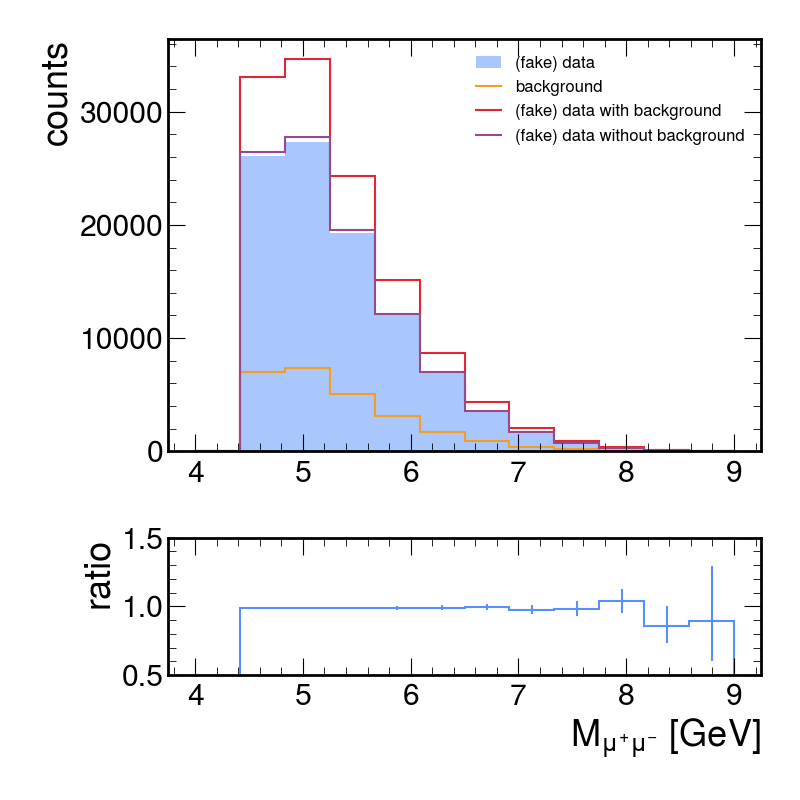
\includegraphics[width=4.5cm]{bs_mass.png}
\end{Pic}

\begin{Pic}{5.}{(5., 0.)}
	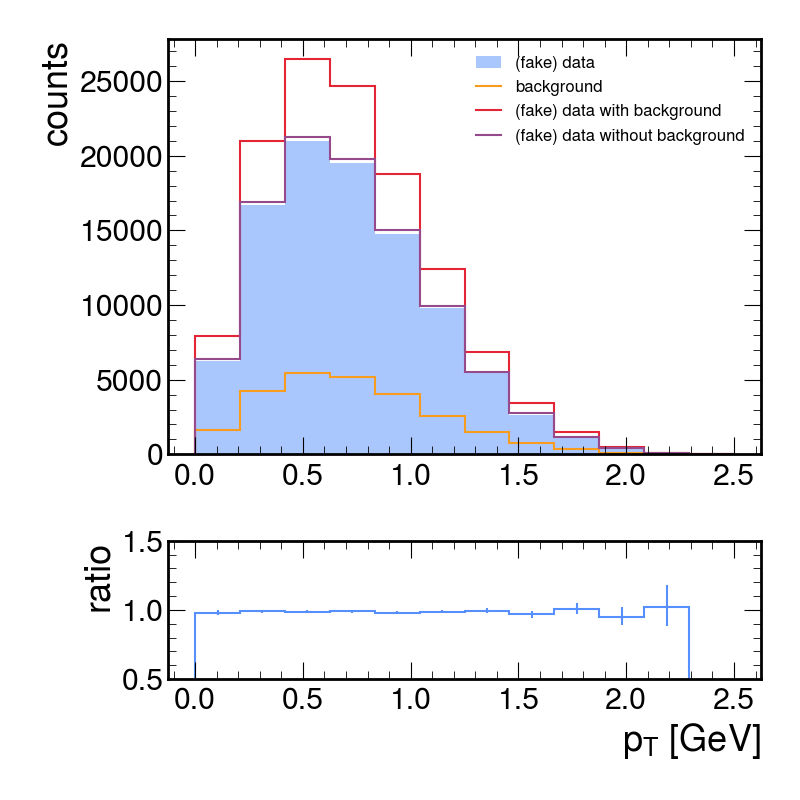
\includegraphics[width=4.5cm]{bs_pT.png}
\end{Pic}

\begin{Pic}{5.}{(10., 0.)}
	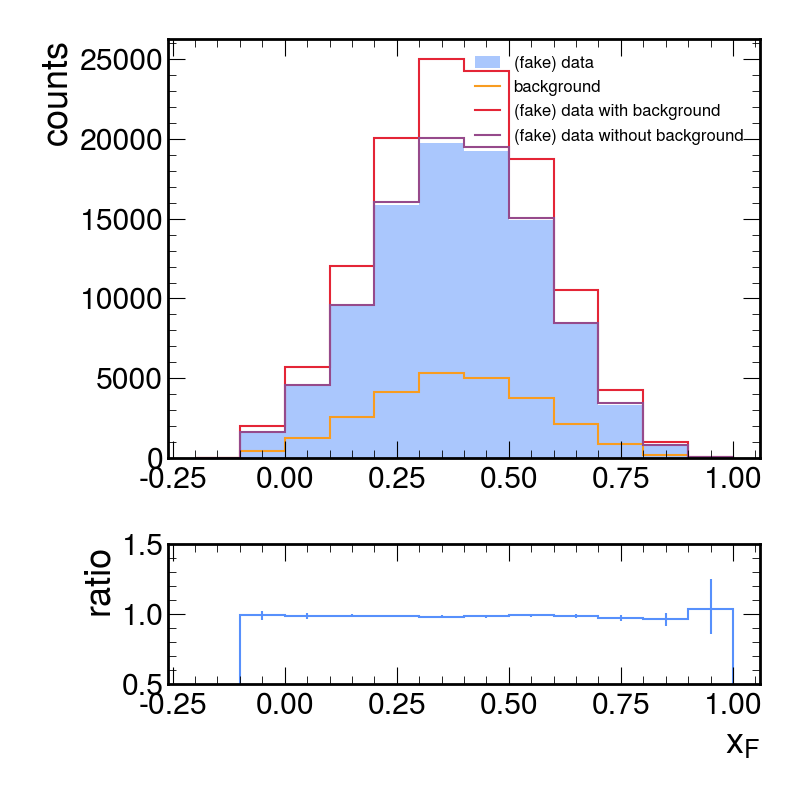
\includegraphics[width=4.5cm]{bs_xF.png}
\end{Pic}

\begin{Pic}{5.}{(0., 7.7)}
	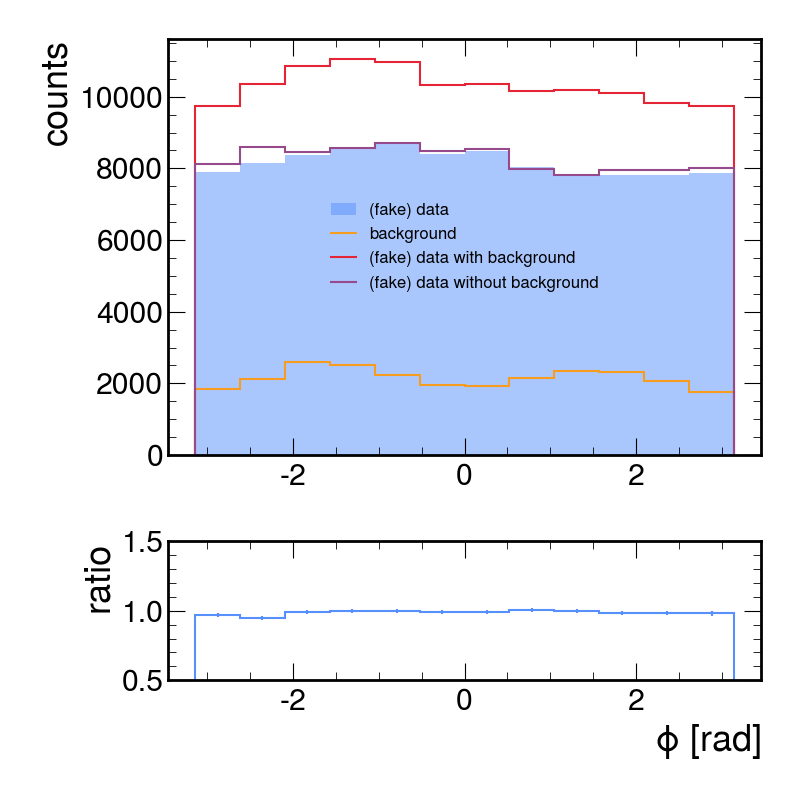
\includegraphics[width=4.5cm]{bs_phi.png}
\end{Pic}

\begin{Pic}{5.}{(5., 7.7)}
	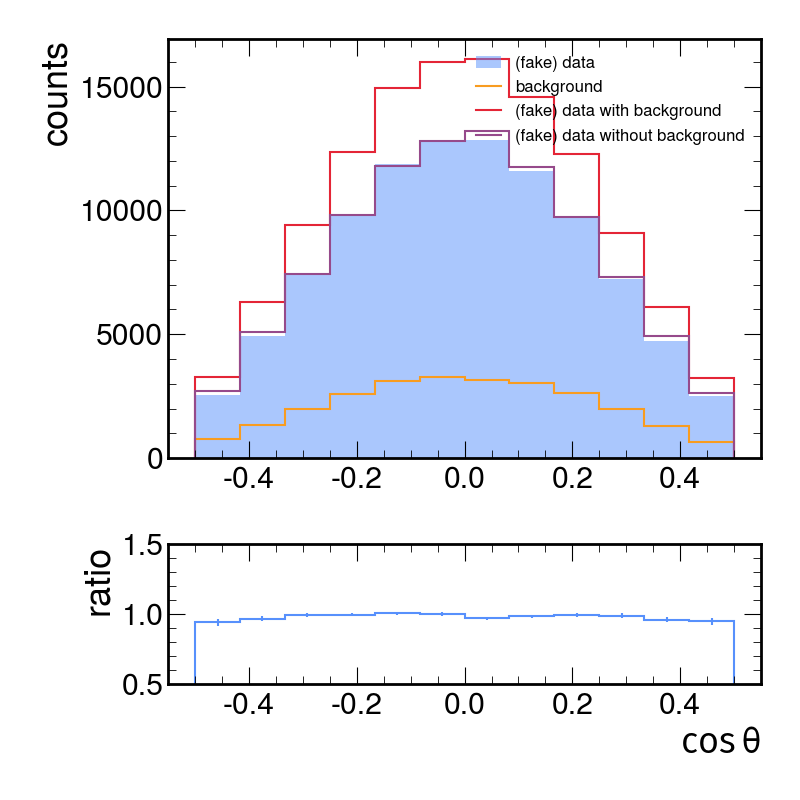
\includegraphics[width=4.5cm]{bs_costh.png}
\end{Pic}

\begin{textblock}{5.}(10., 8.5)
\begin{equation*}
	\omega = \frac{1 - f(x)}{f(x)}
\end{equation*}

$f(x)$ - binary classifier,  $x = [M_{\mu^{+}\mu^{-}}, p_{T}, x_{F}, \phi, \cos\theta]$, 
$x$ - reco. events with background. \\
%Background : $[\lambda, \mu, \nu] = [0.7, -0.2, -0.1]$, \\
%(fake) data $[\lambda, \mu, \nu] = [0.8, 0.1, 0.2]$
\end{textblock}
\end{frame}

\begin{frame}
\frametitle{Unfolding}

\begin{List}{15.}{(0.5, 1.7)}

	\item We use the OmniFold\citeslide{Andreassen:2021zzk} algorithm for unfolding (smearing correction).
	
	\item This is an iterative Bayesian unfolding algorithm that applies ``pushing" and ``pulling" weights between detector-level (reconstructed information) and particle-level (true information).
	
	\item In the first iteration, simulated reconstructed events are reweighted to match the (fake) data at the reconstruction level by classifying the them. The pulling weights, $\omega_{pull}$, are then calculated as,
	
	\begin{equation*}
		\omega_{pull} = \dfrac{1 - f(x_{sim}^{reco.})}{f(x_{sim}^{reco.})}
	\end{equation*}
	
	\item Next, the simulated true events are reweighted to match the weighted ($\omega_{pull}$) simulated true events by classifying them. The pushing weights, $\omega_{push}$, are then calculated as,
	
	\begin{equation*}
		\omega_{push} = \dfrac{1 - f(x_{sim}^{true})}{f(x_{sim}^{true})}
	\end{equation*}
	
	\item These $\omega_{push}$ and $\omega_{pull}$​ weights are updated iteratively.
	
\end{List}
\end{frame}

\begin{frame}

\begin{Pic}{5.}{(0., 0.)}
	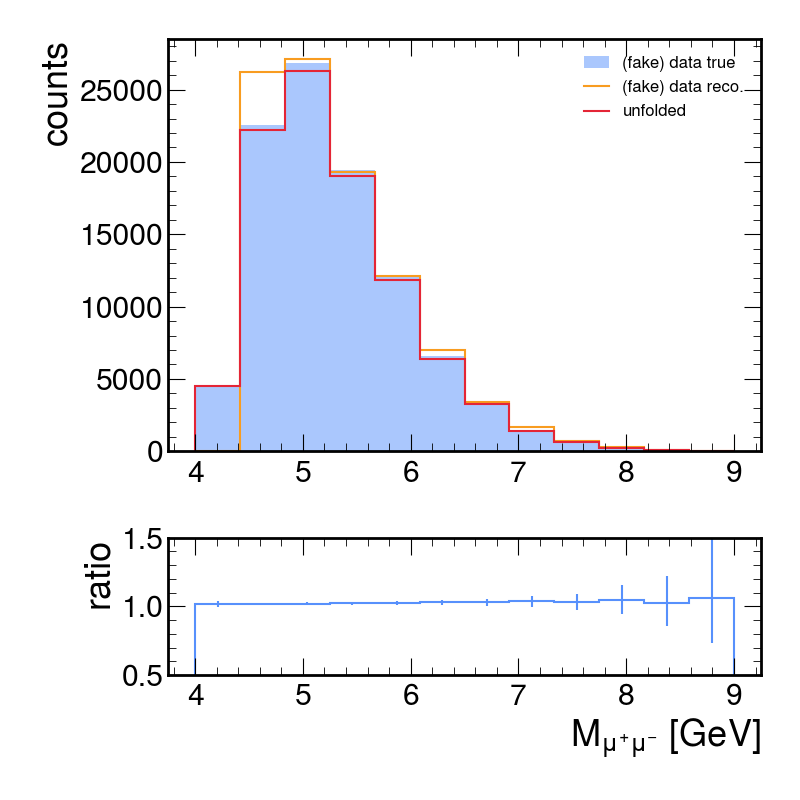
\includegraphics[width=4.5cm]{omnifold_mass.png}
\end{Pic}

\begin{Pic}{5.}{(5., 0.)}
	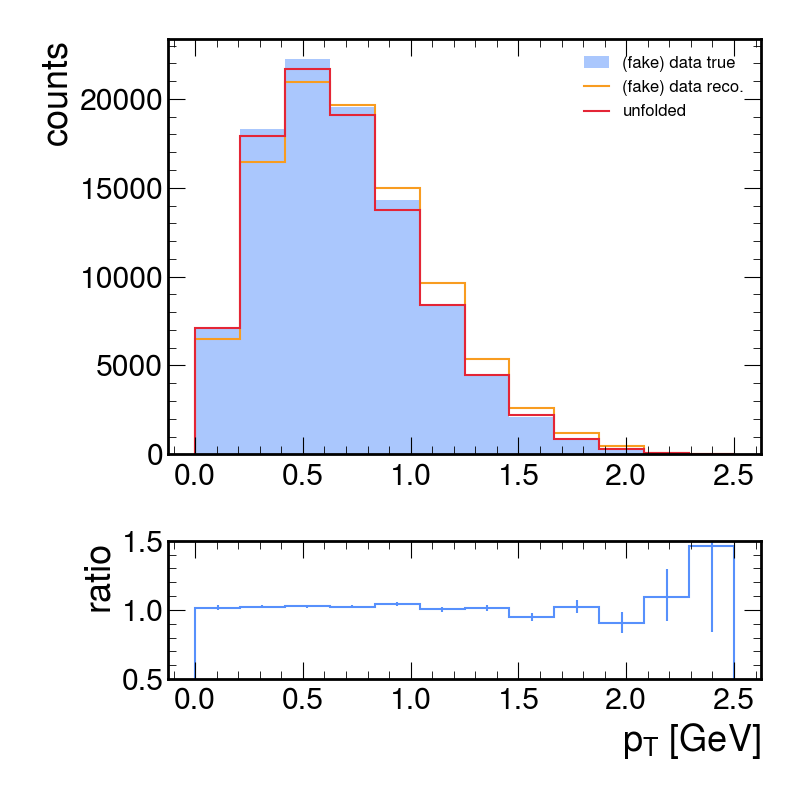
\includegraphics[width=4.5cm]{omnifold_pT.png}
\end{Pic}

\begin{Pic}{5.}{(10., 0.)}
	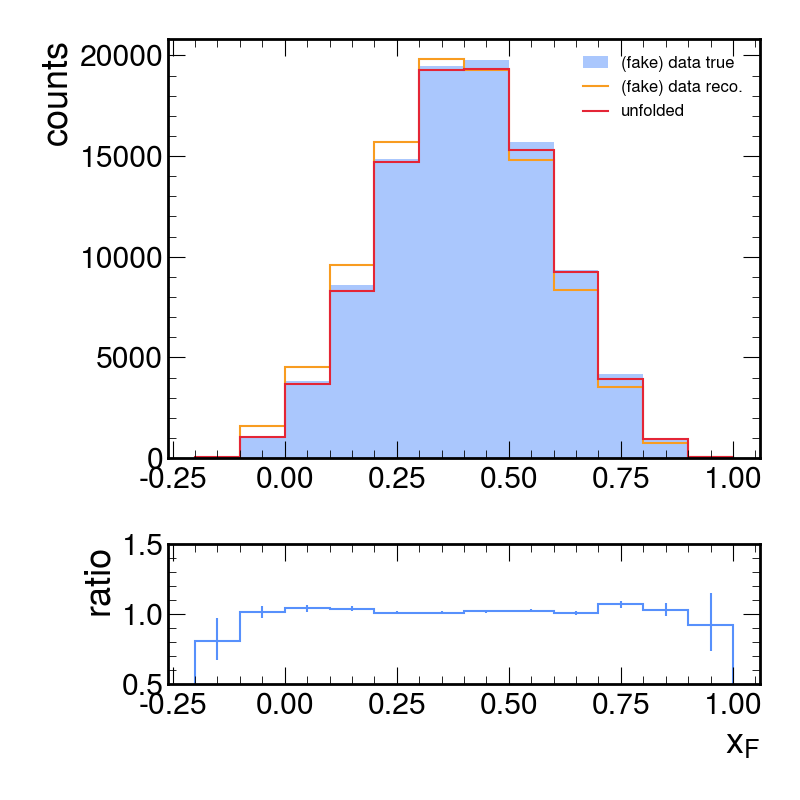
\includegraphics[width=4.5cm]{omnifold_xF.png}
\end{Pic}

\begin{Pic}{5.}{(0., 7.7)}
	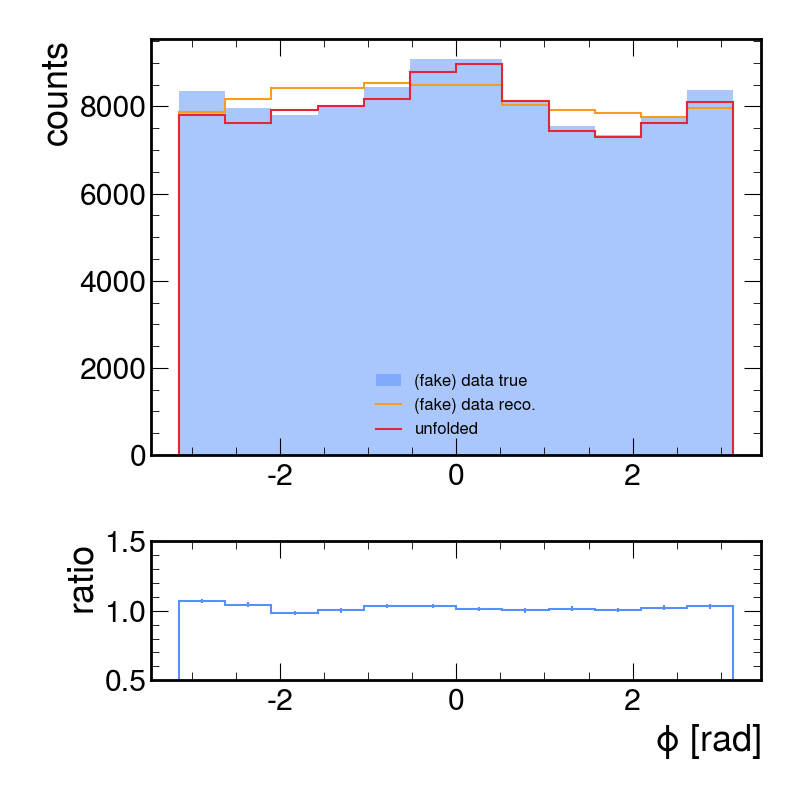
\includegraphics[width=4.5cm]{omnifold_phi.png}
\end{Pic}

\begin{Pic}{5.}{(5., 7.7)}
	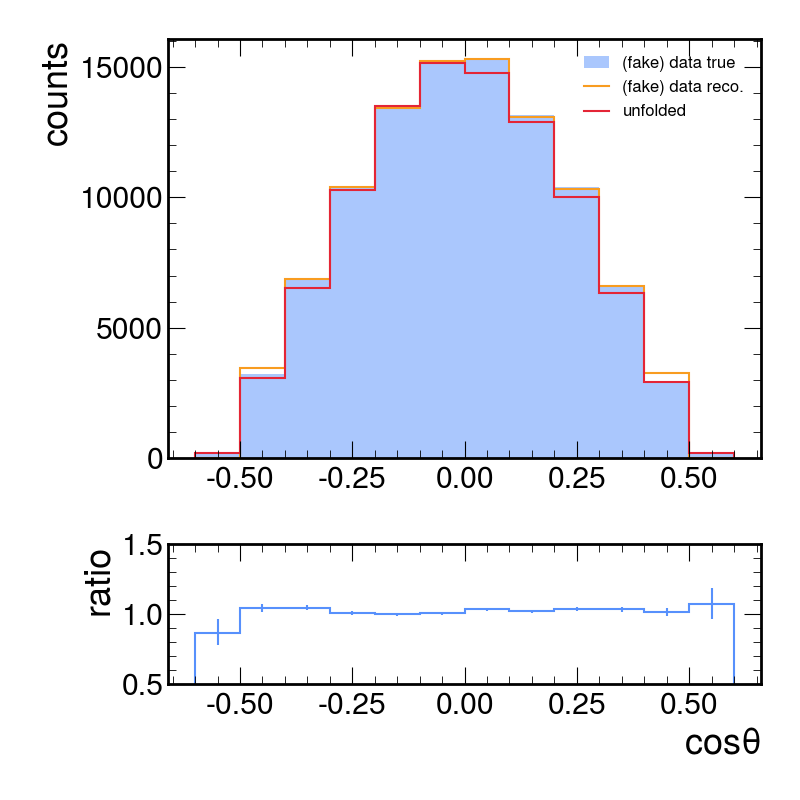
\includegraphics[width=4.5cm]{omnifold_costh.png}
\end{Pic}

\begin{textblock}{5.}(10., 8.5)
\begin{equation*}
	\omega = \frac{1 - f(x_{sim}^{true})}{f(x_{sim}^{true})}
\end{equation*}

$f(x)$ - binary classifier,  $x = [M_{\mu^{+}\mu^{-}}, p_{T}, x_{F}, \phi, \cos\theta]$, 
$x_{sim}^{true}$ - simulated true events.
\end{textblock}

\end{frame}

\begin{frame}
\frametitle{Parameter Inference}

\begin{List}{15.}{(0.5, 2.)}

	\item In this step we want to train a parameterized classifier that can calculate weights for any $\lambda$, $\mu$ and $\nu$. This is achieved by minimizing the loss,\citeslide{Brehmer:2018eca} $^{,}$ \citeslide{Brehmer:2019xox} $^{,}$ \citeslide{Andreassen:2019nnm}
	
	\begin{equation*}
		L[\hat{r}(x | \Theta_{0}, \Theta_{1})] = \dfrac{1}{N}\sum y \left[r(x | \Theta_{0}, \Theta_{1}) - \hat{r}(x | \Theta_{0}, \Theta_{1})\right]^{2} + (1 - y) \left[\dfrac{1}{r(x | \Theta_{0}, \Theta_{1})} - \dfrac{1}{\hat{r}(x | \Theta_{0}, \Theta_{1})}\right]^{2} 
	\end{equation*}
	
	where $x = [\phi, \cos\theta]$, $\Theta = [\lambda, \mu, \nu]$, $[\lambda_{1}, \mu_{1}, \nu_{1}] = [1., 0., 0.]$, 
	
	\begin{equation*}
		r(x|\Theta_{0}, \Theta_{1}) = \dfrac{1 + \lambda_{0}\cos^{2}\theta + \mu_{0}\sin2\theta\cos\phi + \dfrac{1}{2}\nu_{0}\sin^{2}\theta\cos2\phi}{1 + \cos^{2}\theta}
	\end{equation*}
	
	\begin{textblock}{5.}(0.5, 10.)
	\begin{align*}
		\lambda_{0} &\sim \mathcal{U}(-1., 1.) \\
		\mu_{0} &\sim \mathcal{U}(-0.5, 0.5) \\
		\nu_{0} &\sim \mathcal{U}(-0.5, 0.5)
	\end{align*}
	\end{textblock}
	
	\begin{textblock}{5.}(7., 11.)
	\begin{equation*}
		\hat{r}(x|\Theta_{0}, \Theta_{1}) = \dfrac{1 - f(x, \Theta_{0}, \Theta_{1})}{f(x , \Theta_{0}, \Theta_{1})}
	\end{equation*}
	\end{textblock}
	
\end{List}
\end{frame}

\begin{frame}
\frametitle{Parameter Inference}

\begin{List}{15.}{(0.5, 1.5)}

	\item We can train a classifier of the form $f(x, \Theta)$ by classifying the samples ${x, \Theta_{1}}$ with label $y = 1$ and ${x, \Theta_{0}}$ with label $y = 0$.
	
	\item Because $f(x, \Theta)$ is differentiable, it can be used to directly learn and update these parameters during the inference process, allowing us to infer the best parameter.
	
	\item Uncertainties: We found that the variance in the MC events during the training of the parametric model results in large uncertainty. This can be estimated by retraining the parametric model with resampled MC events and using the spread as a source of uncertainty.
\end{List}

\begin{Pic}{5.}{(0., 7.)}
	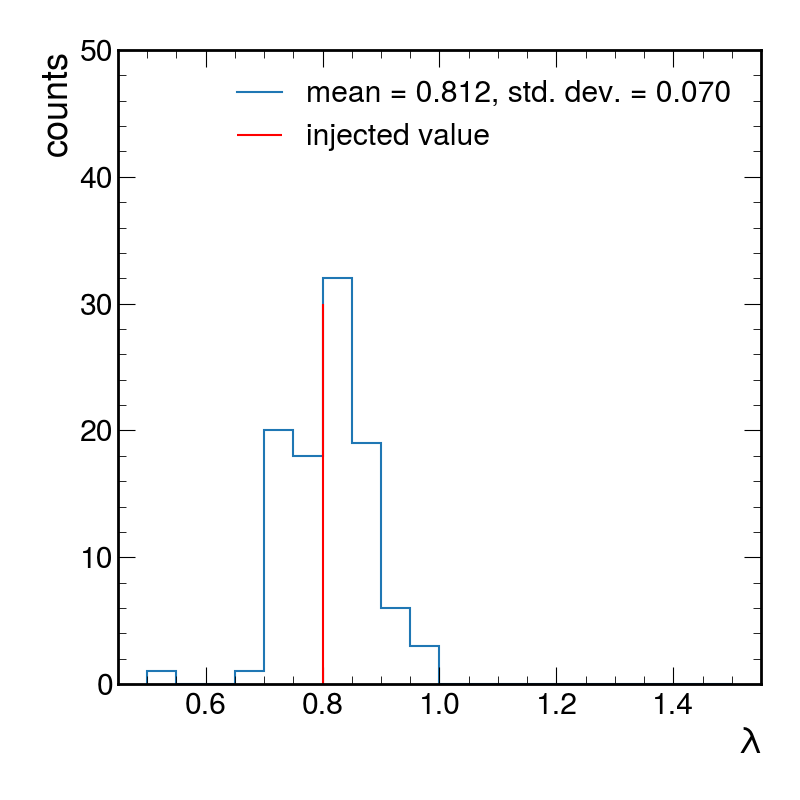
\includegraphics[width=4.9cm]{lambda_var.png}
\end{Pic}
	
\begin{Pic}{5.}{(5., 7.)}
	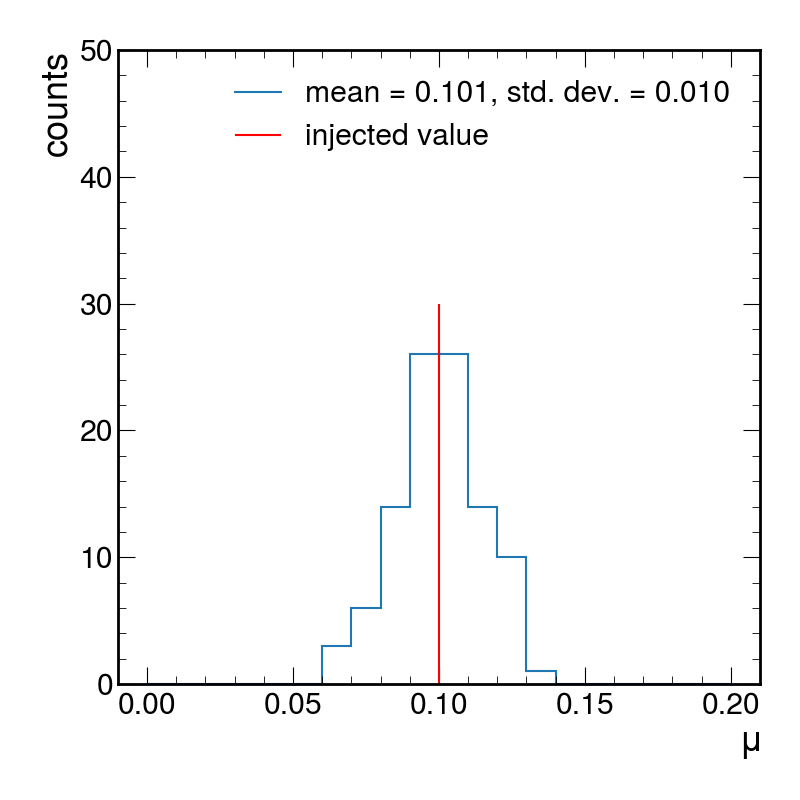
\includegraphics[width=4.9cm]{mu_var.png}
\end{Pic}

\begin{Pic}{5.}{(10., 7.)}
	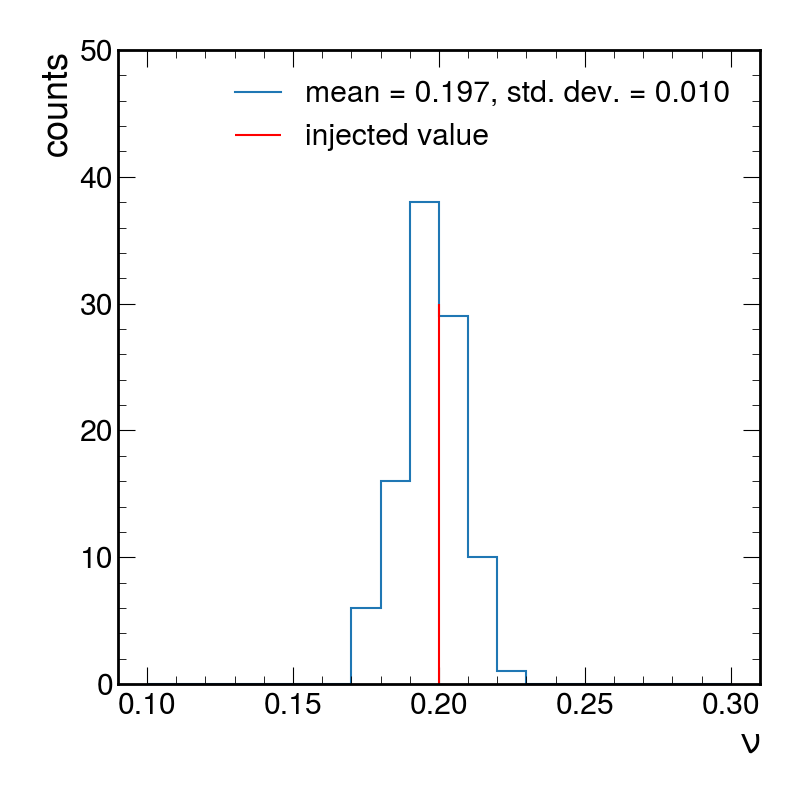
\includegraphics[width=4.9cm]{nu_var.png}
\end{Pic}

%\begin{textblock}{15.}(0.5, 10.)
%	Extracted $\lambda$, $\mu$, and $\nu$ values for 100 models trained with resampled (with replacement) MC events. The mean and standard deviation were calculated for the unbinned values.
%\end{textblock}

\end{frame}

\begin{frame}
\frametitle{Summary}

\begin{List}{15.}{(0.5, 2.)}

    \item The Drell-Yan process is an important experimental approach for exploring the partonic structure of nucleons.
	
	\item A non-zero $\nu$ parameter in the Drell-Yan process provides insights into the transverse motion of quarks within the proton.
	
	\item Deep neural networks based classifiers are ideal candidates for likelihood estimators because of their ability to approximate complex, non-linear functions.
	
	\item Reweighting joint probability distributions is an excellent method for unbinned background subtraction, unfolding, and parameter inference.
	
	\item We are investigating all possible uncertainties in this analysis pipeline.
	
	\item Acknowledgement: This work was supported in part by US DOE grant DE-FG02-94ER40847.
	
\end{List}

\begin{textblock}{15.}(0., 12)
\begin{center}
	Thank You
\end{center}
\end{textblock}

\end{frame}

\end{document}
